\documentclass[twocolumn]{article}
\usepackage[spanish]{babel}
\usepackage[utf8]{inputenc}
\usepackage{amssymb}
\usepackage{graphicx}
\usepackage{verbatim}
\usepackage{algorithmic}
\usepackage{enumitem}
\setlist{nolistsep}




\author{
Nombre:....................................... \\
    Departamento de Informática y Sistemas \\
    Universidad EAFIT \\
}
\title{
    Estructuras de Datos 2 - ST0247 \\
    Supletorio del Examen Parcial 1 
}
\date{
    Septiembre 26 de 2017
}

\begin{document}
\vspace{-5cm}
\maketitle


\section*{Criterios de calificación}

\begin{itemize}
\item Selección múltiple con única respuesta
\begin{itemize}
\item Respuesta correcta: 100\%
\item Respuesta incorrecta: 0\%
\end{itemize}

\item Completar código
\begin{itemize}
\item Respuesta correcta 100\%
\item Respuesta incorrecta o vacía 0\%
\end{itemize}
\end{itemize}

\vspace{1cm}

\textbf{NOTAS IMPORTANTES:}
\begin{itemize}
	\item Responda en la hoja de PREGUNTAS
	\item Marque la hoja de PREGUNTAS
\end{itemize}


\section{Implementación grafos 20\%}
Considere el siguiente grafo:

\begin{center}
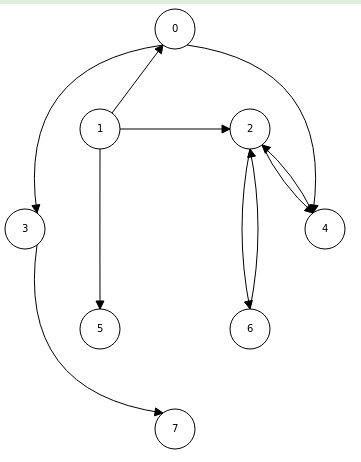
\includegraphics[scale=0.5]{grafin.png}
\end{center}

\begin{enumerate}[label=\Alph*]
	\item (10\%) Complete la representación de \textbf{matrices de adyacencia}. Si no hay arco,
  por simplicidad, deje el espacio en blanco.

\begin{center}
\begin{tabular}{| c | c | c | c | c | c | c | c | c |}
\hline
  & 0 & 1 & 2 & 3 & 4 & 5 & 6 & 7 \\
\hline
0 &   &   &   & 1  & 1  &   &   &   \\
\hline
1 &   &   &   &   &   &   &   &   \\
\hline
2 &   &   &   &   &   &   &   &   \\
\hline
3 &   &   &   &   &   &   &   &   \\
\hline
4 &   &   &   &   &   &   &   &   \\
\hline
5 &   &   &   &   &   &   &   &   \\
\hline
6 &   &   &   &   &   &   &   &   \\
\hline
7 &   &   &   &   &   &   &   &   \\ 
\hline
\end{tabular}
\end{center}

	\item (10\%) Complete la representación de \textbf{listas de adyacencia}. Como
  el grafo no tiene pesos, sólo se colocan los sucesores en la lista de adyacencia.\\


$0 \rightarrow 3 \rightarrow 4$\\
$1 \rightarrow$\\
$2 \rightarrow$\\
$3 \rightarrow$\\
$4 \rightarrow$\\
$5 \rightarrow$\\
$6 \rightarrow$\\
$7 \rightarrow$\\


\end{enumerate}



\section{Recorridos de grafos 20\%}

Para el grafo anterior, complete la salida
que darían los siguientes algoritmos:


\begin{enumerate}[label=\Alph*]
	\item (10\%) Complete el orden en que se recorren los nodos usando \textbf{búsqueda en profundidad} (en Inglés DFS) a partir de cada nodo. Si hay varias opciones de recorrer el grafo con DFS, elija siempre el vértice más pequeño.\\


$0 \rightarrow 3 \rightarrow 7 \rightarrow 4 \rightarrow 2 \rightarrow 6 $\\
$1 \rightarrow$\\
$2 \rightarrow$\\
$3 \rightarrow$\\
$4 \rightarrow$\\
$5 \rightarrow$\\
$6 \rightarrow$\\
$7 \rightarrow$\\


\item (10\%) Complete el orden en que se recorren los nodos usando \textbf{búsqueda en amplitud} (en Inglés BFS) a partir de cada nodo. Si hay varias opciones de recorrer el grafo con BFS, elija siempre el vértice más pequeño.\\


$0 \rightarrow 3 \rightarrow 4 \rightarrow 2 \rightarrow 7 \rightarrow 6 $\\
$1 \rightarrow$\\
$2 \rightarrow$\\
$3 \rightarrow$\\
$4 \rightarrow$\\
$5 \rightarrow$\\
$6 \rightarrow$\\
$7 \rightarrow$\\


\end{enumerate}


\section{Fuerza bruta 20\%}
El problema de encontrar el \textbf{subarreglo máximo} consiste en encontrar un subarreglo contiguo dentro
de un arreglo de números cuya suma sea la máxima. Como un ejemplo, para la secuencia de
números $-2, 1, -3, 4, -1, 2, 1, -5, 4$; el subarreglo contiguo con suma máxima es 
$4, -1, 2, 1$ y su suma es $6$.

El siguiente algoritmo es una solución con fuerza bruta del
problema. El algoritmo consiste en buscar cada posible subarreglo contiguo y luego encontrar la
suma de cada uno de ellos.


\begin{verbatim}
01 int subarregloMax(int[] a) {
02    int maximo = 0;
03    for (int i = 0; i < a.length; i++) {
04       int actual = 0;
05       for (int j = i; j < a.length; j++) {
06          actual = actual + a[j];
07          if (_____________)
08             maximo = actual;
09       }
10    }
11    return maximo;
12 }
\end{verbatim}



\begin{enumerate}[label=\Alph*]


    \item (10\%) Complete el espacio en línea 07


  \_\_\_\_\_\_\_\_\_\_\_\_

      \item (10\%) ¿Cuál es la complejidad asintótica, para el peor de los casos, del algoritmo?


  O(\_\_\_\_)


\end{enumerate}


  % public static int subarregloMax(int[] a)
  % {
  %     int maximo = 0;
  %     for (int i = 0; i < a.length; i++)
  %     {
  %        int actual = 0;
  %        for (int j = i; j < a.length; j++)
  %        {
  %           actual = actual + a[j];
  %           if (actual > maximo)
  %              maximo = actual;
  %        }
  %     }
  %     return maximo;
  % }

\section{Backtracking 30\%}
Un camino hamiltoniano en un grafo dirigido es un camino que visita cada vértice
exactamente una vez. Un \textbf{ciclo hamiltoniano} es un camino hamiltoniano para el cual
existe un arco (en el grafo) que conecta el último vértice del camino hamiltoniano con el primer
vértice del camino hamiltoniano. Su tarea es determinar si dado un grafo, este grafo
contiene un ciclo hamiltoniano o no. Si lo contiene, retorne verdadero; de lo contrario,
retorne falso. 

Parte de su tarea ya está hecha. La función \texttt{sePuede}
verifica si un vértice \texttt{v} se puede agregar al ciclo hamiltoniano
que está almacenado en el arreglo \texttt{path} en la posición \texttt{pos},
dado un grafo representado con matrices de adyancencia \texttt{graph}.
Por simplicidad, sólo se busca si existe un camino que empieza y termina
 en el primer vértice (es decir, en el vértice $0$). Por esta razón, en el arreglo \texttt{path} se entrega con todas sus posiciones en $-1$, excepto
la posición $0$, como se muestra en la función \texttt{cicloHamil}. También, 
por esta razón, en el ciclo de la línea 08, \texttt{v} inicia se con $1$.


\begin{verbatim}
boolean cicloHamil(int graph[][]) {
  path = new int[g.length];
  for (int i = 0; i < g.length; i++)
      path[i] = -1;
  path[0] = 0;
  return cicloHamilAux(graph, path, 1);
}

boolean sePuede(int v, int graph[][], 
                int path[], int pos) {
 if (graph[path[pos - 1]][v] == 0)
    return false;
 for (int i = 0; i < pos; i++)
    if (path[i] == v)
      return false; 
 return true;
}
  
01 boolean cicloHamilAux(int graph[][], 
                   int path[], int pos) {  
02   if (pos == ____________){     
03    if (graph[path[pos-1]][path[0]] == 1)
04           return true;
05    else
06           return false;
07   }
08   for (int v = 1; v < graph.length; v++) {        
09       if (sePuede(__,__,__,__)) {
10           path[pos] = v;
11           if (cicloHamilAux(__,__,__))
12               return true;
13           path[pos] = -1;
14       }
15   }
16   return false;
17 }
\end{verbatim}


\begin{enumerate}[label=\Alph*]


    \item (10\%) Complete el espacio en línea 02 que corresponde a la condición de parada


  \_\_\_\_\_\_\_\_\_\_\_\_


    \item (10\%) Complete los espacios en línea 09 que corresponden al llamado de la función sePuede


  \_\_\_\_\_\_\_\_, \_\_\_\_\_\_\_\_, \_\_\_\_\_\_\_\_, \_\_\_\_\_\_\_\_


    \item (10\%) Complete los espacio en la línea 11 que corresponden al llamado recursivo de la función cicloHamil


  \_\_\_\_\_\_\_\_, \_\_\_\_\_\_\_\_, \_\_\_\_\_\_\_\_



\end{enumerate}

% boolean sePuede(int v, int graph[][], 
%                 int path[], int pos) {
%         if (graph[path[pos - 1]][v] == 0)
%             return false;
%         for (int i = 0; i < pos; i++)
%             if (path[i] == v)
%                 return false; 
%         return true;
% }
  
% 01 boolean cicloHamil(int graph[][], 
%                    int path[], int pos) {  
% 02        if (pos == graph.length){     
% 03            if (graph[path[pos - 1]][path[0]] == 1)
% 04                return true;
% 05            else
% 06                return false;
% 07        }
% 08        for (int v = 1; v < graph.length; v++) {        
% 09            if (sePuede(v, graph, path, pos)) {
% 10                path[pos] = v;
% 11                if (cicloHamil(graph, path, pos + 1))
% 12                    return true;
% 13                path[pos] = -1;
% 14            }
% 15        }
% 16        return false;
% 17 }

\section{Alg. Voraces 10\%}

El problema de \textbf{selección de actividades} consiste en encontrar el máximo número de actividades que una persona o una máquina puede resolver, asuminedo que la persona o máquina sólo puede hacer una actividad al mismo tiempo. Este problema es de interés en
Ingeniería de Producción. Cada actividad tiene un tiempo de inicio y un tiempo de fin. Como un ejemplo, considere las siguientes actividades:\\

\begin{tabular}{| l | l | l | l | l | l | l | l | l |}
\hline
Act. &	a1 &	a2 &	a3 &	a4 &	a5& 	a6& 	a7 &	a8\\
\hline
inicio &	1 &	0 &	1 &	4 &	2 &	5 &	3 &	4 \\
fin &	3 &	4 &	2 &	6 &	9 &	8 &	5 &	5 \\ 
\hline
\end{tabular}\\

Nuestra tarea es encontrar el máximo número de actividades que se puedan ejecutar y que no estén en conflicto (es decir, que no ocurran dos al mismo tiempo). 
Un algoritmo voraz para resolver el problema funciona de la siguiente forma: 

\begin{enumerate}
  \item Ordenar las actividades de menor a mayor, según el tiempo de fin de la actividad
  \item Seleccionar la primera actividad
  \item Repetir hasta que no se puedan seleccionar más actividades: 
  \begin{itemize}
    \item Seleccionar una nueva actividad cuyo tiempo de inicio sea mayor igual al tiempo de fin de la actividad previamente seleccionado.
  \end{itemize}
\end{enumerate}

Para el ejemplo anterior, el algoritmo debe entregar la siguiente
respuesta:\\

\begin{center}
\begin{tabular}{| l | l | l |}
\hline
  Actividad   &   Inicio   &  Fin\\
  \hline
        a3     &     1    &      2\\
        a7     &     3    &      5\\
        a6      &    5     &     8\\ 
        \hline
\end{tabular}\\
\end{center}

A continuación observamos una implementación del algoritmo en Java:

{\small
\begin{verbatim}
class Actividad {
  public Actividad(String a,int b,int c) {
      id = a; inicio = b; fin = c;}
  String id;
  int inicio;
  int fin;
}
void seleccion(Actividad actividades[]) {
  int i, j;
  int n = actividades.length;
  Actividad temp;
  //paso 1
  for(i = 1; i < n; i++) {
    for(j = 0; j < n - 1; j++){
      if(actividades[j].fin > actividades[j+1].fin) {
        temp = actividades[j];
        actividades[j] = actividades[j+1];
        actividades[j+1] = temp;
      }
    }
  }
  //paso 2
  System.out.println("Actividad Inicio Fin");
  System.out.println(actividades[0].id + " " + 
                     actividades[0].inicio + " " +  
                     actividades[0].fin);
  //paso 3
  i = 0;
  for(j = 1; j < n; j++) {
    if(actividades[j].inicio >= actividades[i].fin) {
      System.out.println(actividades[j].id + " " +  
                         actividades[j].inicio + " " +  
                         actividades[j].fin);
      _________
    }
  }

\end{verbatim}
}

Complete el espacio faltante en la última línea \\

	\_\_\_\_\_\_\_\_\_\_\_\_\_\_\_\_\_\_\_\_\_\_\_\_

% i = j






\end{document}